\documentclass[UTF8,a4paper,8pt]{ctexart} 

 \usepackage{graphicx}%学习插入图
 \usepackage{verbatim}%学习注释多行
 \usepackage{booktabs}%表格
 \usepackage{geometry}%图片
 \usepackage{amsmath} 
 \usepackage{amssymb}
 \usepackage{listings}%代码
 \usepackage{xcolor}  %颜色
 \usepackage{enumitem}%列表格式
 \CTEXsetup[format+={\flushleft}]{section}


\geometry{left=1.6cm,right=1.8cm,top=2cm,bottom=1.7cm} %设置文章宽度

\pagestyle{plain} 		  %设置页面布局
\author{\kaishu 郑华}
\title{\heiti Python }
%代码效果定义
\definecolor{mygreen}{rgb}{0,0.6,0}
\definecolor{mygray}{rgb}{0.5,0.5,0.5}
\definecolor{mymauve}{rgb}{0.58,0,0.82}
\lstset{ %
	backgroundcolor=\color{white},   % choose the background color
	basicstyle=\footnotesize\ttfamily,        % size of fonts used for the code
	%stringstyle=\color{codepurple},
	%basicstyle=\footnotesize,
	%breakatwhitespace=false,         
	%breaklines=true,                 
	%captionpos=b,                    
	%keepspaces=true,                 
	%numbers=left,                    
	%numbersep=5pt,                  
	%showspaces=false,                
	%showstringspaces=false,
	%showtabs=false,        
	columns=fullflexible,
	breaklines=true,                 % automatic line breaking only at whitespace
	captionpos=b,                    % sets the caption-position to bottom
	tabsize=4,
	commentstyle=\color{mygreen},    % comment style
	escapeinside={\%*}{*)},          % if you want to add LaTeX within your code
	keywordstyle=\color{blue},       % keyword style
	stringstyle=\color{mymauve}\ttfamily,     % string literal style
	frame=single,					%tb top and bottom; L left double line
	xleftmargin=.06\textwidth, 
	%xrightmargin=.1\textwidth,
	rulesepcolor=\color{red!20!green!20!blue!20},
	% identifierstyle=\color{red},
	language=python,
}

\begin{document}          %正文排版开始
 	\maketitle
  
  \newpage
  \section{安装与系统环境变量配置}
	  \paragraph{1.环境变量}为了在命令行dos 下能执行python命令,需要将python.exe 文件的目录添加到path 中
  
  \newpage
  \section{基础编程}
	  \paragraph{Basic}
		  \begin{itemize}
			  	\item 注释:以\# 开头的语句是注释
			  	\item 语法:当语句以冒号:结尾时,缩进的语句视为代码块,应该始终坚持使用4个空格的缩进
			  	\item 大小写区分
		  \end{itemize}
	  
	  \paragraph{数据类型和变量}
	  
		  \begin{itemize}
			  	\item  整数: 十六进制用0x前缀和0-9,a-f表示,如0xa5b4c3d2
			  	\item  浮点数: 1.23x$10^9$就是1.23e9
			  	\item  字符串: 以单引号'或双引号"括起来的任意文本,比如'abc',"xyz",字符串内部有很多换行,用'''...'''的格式表示多行内容
				  	\begin{lstlisting}
	>>> print('''line1
	... line2
	... line3''')
	#line1
	#line2
	#line3			  		
				  	\end{lstlisting}
			  	\item  布尔: True、 False  注意大小写,运算包括 and, or, not
			  	\item  空值: 用None表示, None不能理解为0,因为0是有意义的,而None是一个特殊的空值
			  	\item  变量: 变量名必须是大小写英文、数字和\_的组合,且不能用数字开头
			  	
					  \begin{enumerate}
					  	\item 动态变量:可以把任意数据类型赋值给变量,同一个变量可以反复赋值,而且可以是不同类型的变量
						  	\begin{lstlisting}
	a = 123 # a是整数
	print(a)
	a = 'ABC' # a变为字符串
	print(a)						  	
						  	\end{lstlisting}
					  	\item 静态变量:在定义变量时必须指定变量类型,如果赋值的时候类型不匹配,就会报错,这个例如C++,\textit{但是python是动态变量}
					  	
					  	\item 变量赋值:把一个变量a赋值给另一个变量b
						  	\begin{lstlisting}
	a = 'ABC'
	b = a
	a = 'XYZ'
	print(b)					  		
						  	\end{lstlisting}
						  	\begin{itemize}
						  		\item 执行a = 'ABC',解释器创建了字符串'ABC'和变量a,并把a指向'ABC':
							  		\begin{figure}[h]
							  			\centering
							  			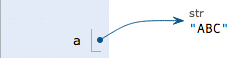
\includegraphics[scale=.5]{python-png/01.png}
							  		\end{figure}
						  		\item 执行b = a,解释器创建了变量b,并把b指向a指向的字符串'ABC':
							  		\begin{figure}[h]
							  			\centering
							  			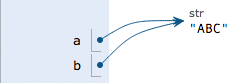
\includegraphics[scale=.5]{python-png/02.png}
							  		\end{figure}
						  		\item 执行a = 'XYZ',解释器创建了字符串'XYZ',并把a的指向改为'XYZ',但b并没有更改:
							  		\begin{figure}[h]
							  			\centering
							  			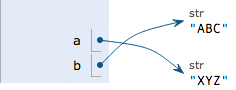
\includegraphics[scale=.5]{python-png/03.png}
							  		\end{figure}
						  	\end{itemize}
						  	
					  \end{enumerate}
				\item  常量:通常用全部大写的变量名表示常量
				\item  除法:/ 表示精确除法; //表示去小数除法,得到一个整数
		  \end{itemize}
	\paragraph{List 与 Tuple}     
\end{document} 
 		    